\documentclass[a4paper,11pt]{report}
\usepackage[T1]{fontenc}
\usepackage[utf8]{inputenc}
\usepackage{lmodern}
\usepackage[spanish]{babel}
\usepackage{graphicx} % para insertar graficos/imagenes
\usepackage{float} % me deja usar la H de 'here' en los graficos para ponerlos donde yo quiera
\usepackage{enumerate}
\usepackage{fancyhdr} % headers y footers
\usepackage{color} %Para colores y eso
\usepackage{geometry} %Para cambiar la geometria de las hojas
\usepackage{multirow} % para las tablas
 \usepackage[hidelinks]{hyperref} 
\let\olditemize\itemize
\def\itemize{\olditemize\itemsep=0pt }

\title{Trabajo Practico: Fine Food Reviews\\Organización de Datos 75.06}
\author{Joaquín Blanco, Padrón: 94653\\
Joaquín Casal, Padrón: 98280\\
Franco Etcheverri, Padrón: 95812\\
Agustín Luques, Padrón: 96803\\
Nombre del grupo en Kaggle: Tony Spark}

\begin{document}

\maketitle
\tableofcontents

\begin{abstract}
En el presente documento se propone explicar la forma en la cuál se llevo adelante la resolución del trabajo práctico y todas las opciones evaluadas durante el desarrollo del mismo. 

La base de las ideas que fueeon presentadas en el informe de diseño son las mismas sobre las cuales se sustentan nuestros algoritmos finales. En las siguientes secciones se desarrollaran en mayor detalle los cambios y mejoras que se implemetaron.

En términos generales, para la resolución del problema planteado se utilizan dos algoritmos principales:

\begin{itemize}
    \item Algoritmo de estilo probabilistico (Adaptación de Naive Bayes)
    \item Algoritmo de K-Means
\end{itemize} 

Ambos algoritmos son independientes uno del otro y generan su propia predicción sobre la review. Por este motivo y con el objetivo de llegar a una precisión mayor se desarrollar una serie de combiners los cuales a partir de los dos resultados generasen uno nuevo como valor final.
\end{abstract}

\chapter{Análisis inicial de los datos}

Como bien se planteo desde un principio el campo principal sobre el cual ibamos a enfocar nuestro desarrollo era el de texto. Las principales diferencias con respecto al diseño son que, luego de estudiar nuevamente el set de datos, consideramos que los "Helpfullnes Numbers" no iban a servir para la tarea que teníamos que llevar adelante. Dichos campos serían más apropiadas para un caso en el cual hubiesemos tenido que otorgarle un puntaje al producto y no a la review. En dicho caso estos valores hubieran jugado un rol importante, pero para nuestro análisis fueron descartados.

En resumen, los únicos campos que tomamos en cuenta, obviamente además de la predicción del set de training, fueron el text y el summary.





%Para tener una primer idea de los posibles resultados, analizamos la cantidad de %registros por cada valor posible de estrellas y lo que obtuvimos se puede observar %en la Figura \ref{fig:2}. 

%\begin{figure}[htp]
%  \begin{center}
%    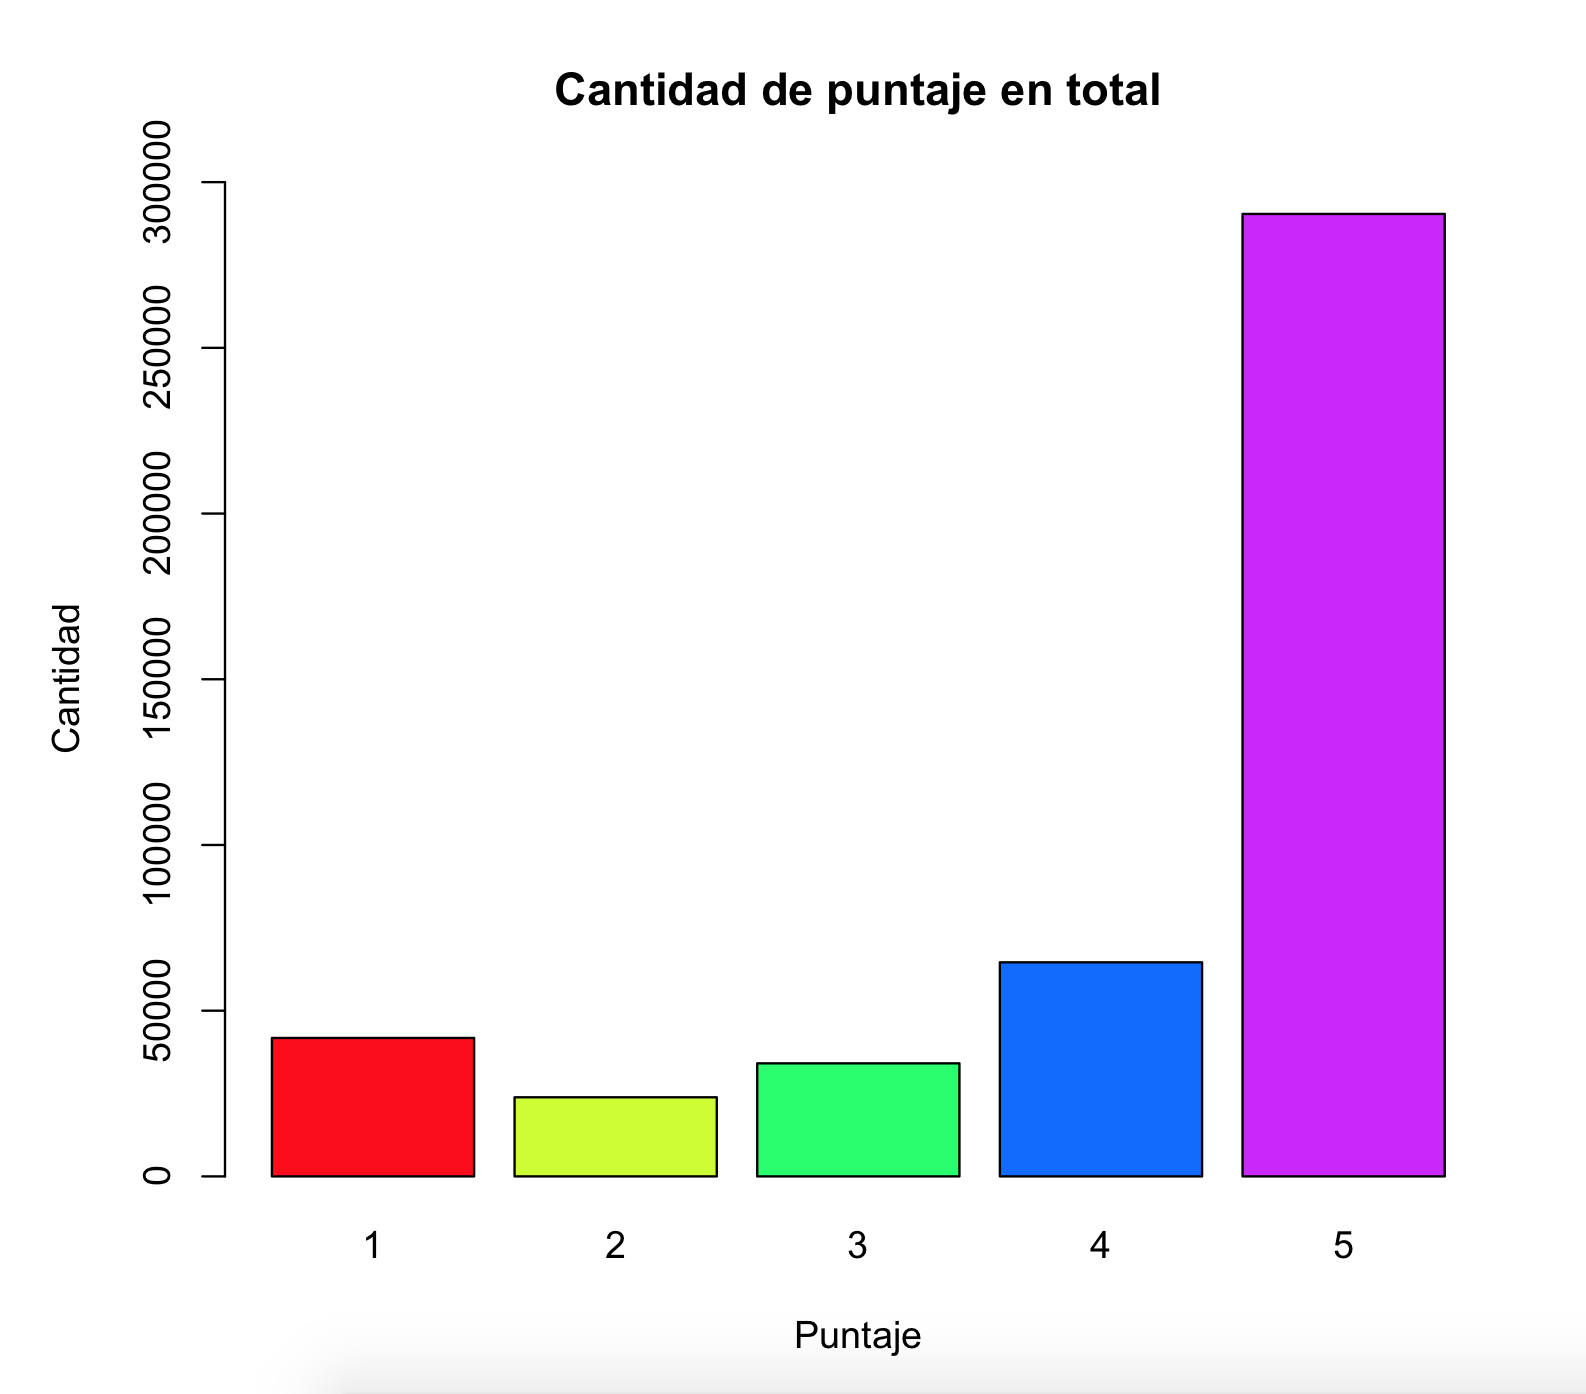
\includegraphics[width=10cm]{puntajcant}
%    \caption{Frecuencia de los distintos puntajes}
%    \label{fig:2}
%  \end{center}
%\end{figure}


\chapter{Transformando los datos}

Como bien se presento en el diseño, la idea era pre procesar los textos para quedarnos únicamente con aquellas palabras que mejoraran el aprendizaje del algoritmo y aseguraran un correcto funcionamiento. 

La diferencia frente a lo planteado inicialmente es que las únicas palabras que afectaran la predicción final son los adjetivos por lo que al resto no se les va a calcular un puntaje asociado. Para ello se utilizó una lista de adjetivos en ingles. 


\chapter{Algoritmo de estilo probabilistico (Adaptación de Naive Bayes)}

La clasificación de Bayes consiste en asignarle la clase con mayor probabilidad a un ejemplo determinado a partir de su contenido. Para adaptar el algoritmo a nuestro trabajo lo que se busco es extender la posibilidad de clasificación más alla de las clases sobre las que partimos, en nuestro caso la cantidad de estrellas del review del 1 al 5. Para ello, y con el objetivo de aceptar valores no enteros como resultado, se propuso obtener la predicción a traves de un promedio de los puntajes asociados a cada palabra, más precisamente adjetivo, de la review.

Los pasos del algoritmo son los siguientes:

\begin{enumerate}[1.]
    \item Crear un diccionario inicialmente vacio y una lista con las palabras de negación en ingles (Ej: not, isnt).
    
    \item Abre un archivo de texto en el cual se encuentran guardados todos los adjetivos que vamos a considerar.
    
    \item Se va guardando en el diccionario los adjetivos y adicionalmente una combinación de negacion+adjetivo (concatenados) para cada adjetivo y cada palabra de la lista de negaciones.
    
    \item Abre el archivo de train (Previamente pre procesado) y para cada fila únicamente toma el campo número nueve y diez que son el texto y el resumen.
    
    \item Toma cada palabra de los campos anteriores y si ésta se encuentra en el diccionario creado, se la agrega a una nueva lista de la siguiente forma: (Puntaje del review actual, palabra).
    
    \item Se genera un RDD con la lista completa de palabras con sus respectivos puntajes.
    
    \item Map para darle el siguiente formato a los datos: (Palabra, (1, puntaje)).
    
    \item ReduceByKey para obtener la cantidad de veces que aparece cada palabra junto con la suma de puntajes de los reviews en las cuales aparece.
    
    \item A través de otro Map se obtiene el puntaje promedio de cada palabra: (Palabra, Puntaje Promedio).
    
    \item Abre el archivo de Test (Previamente pre procesado) y coloca en un RDD (ID Review, texto)
    
    \item Separa cada palabra del campo texto para lograr el siguiente formato: (Palabra, ID)
    
    \item A traves de un leftOuterJoin entre los dos RDDs se logra generar la tupla (Palabra, (ID, Puntaje)) en el caso de que la palabra se encuentre en el RDD de train y (Palabra, (ID, none)) en caso contrario.
    
    \item Se elimina el campo de palabra del RDD.
    
    \item Map para lograr (ID, (Puntaje, 1)).
    
    \item ReduceByKey para obtener la cantidad de palabras consideradas para predecir el puntaje junto con el puntaje total obtenido de la suma del de cada palabra.
    
    \item Map para lograr el formato de predicción correspondiente: (ID, Puntaje Promedio).
    
\end{enumerate}

\chapter{K-means y Knn}


\chapter{Combinación de clasificadores}

Para lograr combinar los resultados de cada algoritmo independiente, se utilizaron los siguientes métodos de combiners:

\begin{itemize}
    \item Promedio
    \item Promedio ponderado
\end{itemize} 

Para el caso del promedio ponderado, se utilizó un factor de fiabilidad para darle mayor importancia a la predicción de uno u otro algoritmo.

Para obtener el valor de fiabilidad se procedió a separar una porción del train y dejarla fuera del entrenamiento de los algoritmos para luego poder evaluar que tan preciso son los mismos. 

A partir de los resultados obtenidos y normalizando los valores para que la suma de los dos factores de fiabilidad (uno para cada algoritmo) de igual a uno, se procedio a calcular la predicción final como:

\[ Predicción = \ C_{1} . Predicción_{1} + C_{2} . Predicción_{2} \]


\chapter{Tabla de Submits de Kaggle}

\begin{table}[htbp]
\begin{center}
\begin{tabular}{|l|l|l|}
\hline
Submit & Descripción & Resultado \\
\hline \hline \hline
1 & Bayes: sin juntar negaciones & 1.48598 \\ \hline
2 & Bayes: juntando negaciones & 1.46913  \\ \hline
3 & Bayes: agregamos campo summary, valor por default 4.5 & 1.38063 \\ \hline
4 & Bayes: agregamos campo summary, valor por default 4.0 & 1.37189 \\ \hline
5 & Bayes: agregamos campo summary, valor por default 3.0 & 1.37214 \\ \hline
\end{tabular}
\caption{Tabla muy sencilla.}
\label{tabla:sencilla}
\end{center}
\end{table}

\chapter{Comentarios}

La idea de tener que predecir en funcion de lo que un usuario escribe nos resulto muy interesante pero a la vez un desafio algo dificil, más que nada por el hecho de que las personas muchas veces realizan errores de tipeo o tienen faltas de ortografía que si bien son pequeños detalles, en cuanto a la forma de detectarlos y evitar que jueguen un papel negativo importante en el desarrollo de nuestros algoritmos es algo vital y bastante dificil de solucionar por completo. 

Por otro lado, nos resulto sorprendete la inmensa variedad de enfoques que se le pueden dar a temas relacionados con text mining. Ya que más alla de los algoritmos que elegimos nosotros, en la parte previa de estudio y diseño del TP fuimos discutiendo y evaluando muchos más.

Los resultados creemos que son positivos, evauando el tiempo acotado que se tiene en solo un cuatrimestre y la poca experiencia de nuestra parte para con estos temas en un principio, el saldo final es bueno.

En conclusión fue un trabajo interesante y llevadero, el cual si bien es complicado y lleva su tiempo, conlleva consigo mucho aprendizaje y satisfacción a la hora de ver los resultados obtenidos.  

\begin{thebibliography}{99}
\bibitem{Opinion} Bing Liu, Lei Zhang. A Survey of Opinion Mining and Sentiment Analysis, Capitulo del libro Mining Text Data. Ed. C. Aggarwal, C. Zhai, Springer, 2011.
\bibitem{Comb1} Leah S. Larkey, W. Bruce Croft. Combining Classifiers in text categorization. Departamento de Ciencias de la Computacion. Universidad de Massachusetts.
\bibitem{Poco} Daphne Koller, Mehran Sahami. Hierarchically classifying documents with very few words. Departamento de Ciencias de la Computacion. Universidad de Stanford
\bibitem{mining} Editors: Aggarwal, Charu C., Zhai, ChengXiang (Eds.). Mining Text Data
\bibitem{Com2} Paul N. Bennett, Susan T. Dumais, Eric Horvitz. Probabilistic Combination of Text Classifiers Using Reliability Indicators: Models and Results.
\bibitem{Mining2}Ronen Feldman, James Sanger. The Text Mining Handbook.
\bibitem{Mining3} Kunpeng Zhang, Yu Cheng, Wei-keng Liao, Alok Choudhary. Mining Millions of Reviews: A Technique to Rank Products Based on Importance of Reviews. Universidad de Northwestern.
\bibitem{apunte} Luis Argerich, Apuntes del Curso Organización de Datos.
\bibitem{link1} Data Science in Minutes. 
\url{ https://rdisorder.wordpress.com/2016/08/06/data-science-in-minutes/}
\bibitem{link2} All About Stop Words for Text Mining and Information Retrieval. 
\url{http://text-analytics101.rxnlp.com/2014/10/all-about-stop-words-for-text-mining.html}
\bibitem{link3} Clasificador bayesiano ingenuo. 
\url{https://es.wikipedia.org/wiki/Clasificador_bayesiano_ingenuo}
\end{thebibliography}

\end{document}
